\chapter{المتريات، والتمدد، ومدخل أول إلى علم الكونيات}

في نهاية المحاضرة السابقة كنا قد وصلنا إلى معادلة موجية ثابتة تحت تحولات لورنتز، وكنا نستعد لكتابة معادلات ماكسويل بصيغة الزمكان. ويقدم لنا الآن سؤال من الحضور تنبيهًا مفيدًا قبل أن ننتقل إلى الثقالة: إلى أي حد يستطيع التناظر، بذاته، أن يحدد نظرية فيزيائية؟ والجواب قاطع: إلى حد كبير، ولكن ليس كل شيء. إن ثبات لورنتز مرشِّح قوي للقوانين الممكنة. لكنه ليس بديلًا عن الافتراضات الفيزيائية المتبقية ولا عن التجربة.

\section{ما لا يحدده التناظر}

\begin{classroomqa}
\audiencequestion{بعد أن نعلم أن المجالين الكهربائي والمغناطيسي يتحولان معًا تحت تحولات لورنتز، فهل تتبع معادلات ماكسويل من النسبية وحدها؟}
\lecturerresponse{لا. فالنسبية تقيِّد صورة المعادلات، لكن بناءها يستخدم أيضًا خطيتها، وانخفاض رتبة مشتقاتها، والطريقة التي تتحول بها الحقول، ومعلومات تجريبية. ومن دون تلك العناصر الإضافية تظل معادلات حقلية كثيرة متغايرة لورنتزيًا ممكنة.}
\end{classroomqa}

أهم تلك الافتراضات الإضافية في المناقشة الافتتاحية هو الخطية. فإذا كانت \(A(x,t)\) حلًا لمعادلة حقلية خطية، فإن \(\lambda A(x,t)\) يكون أيضًا حلًا لأي ثابت \(\lambda\). وإذا كان كل من \(A\) و\(B\) حلًا، فإن \begin{equation}
  C(x,t)=A(x,t)+B(x,t).
  \label{eq:superposition}
\end{equation}
وهذا هو مبدأ التراكب. يمكن لموجتين كهرومغناطيسيتين خاليتين من المصادر أن تعبر إحداهما الأخرى وتخرجا من ذلك بلا تغير. فهما لا تتصادمان مباشرة على النحو الذي تفعله الأجسام المادية. ويمكنهما أن تتفاعلا على نحو غير مباشر عبر مادة مشحونة، لأن كل موجة تحرك الشحنات، والشحنات المتحركة تشع، لكن معادلات الحقل في الفراغ نفسها خطية.

\begin{figure}[H]
\centering
\includegraphics[width=0.64\textwidth]{lecture_08_figure_01.png}
\caption{منحنيان لموجتين على اللوح أثناء مناقشة التراكب. ومجموعهما هو أيضًا موجة خالية من المصادر مسموح بها.}
\lectureframe{00:05:30}
\end{figure}

يوضح المهتز التوافقي الجبر بجلاء. لنفترض
\begin{equation}
  m\ddot x=-kx.
  \label{eq:linear-oscillator}
\end{equation}
إذا كان \(x_1\) و\(x_2\) يحلان \eqref{eq:linear-oscillator}، فإن
\begin{equation}
  m(\ddot x_1+\ddot x_2)
  =-k(x_1+x_2),
\end{equation}
ولذلك يكون \(x_1+x_2\) حلًا. لكن إذا أضفنا حدًا لاخطيًا،
\begin{equation}
  m\ddot x=-kx+p x^2,
  \label{eq:nonlinear-oscillator}
\end{equation}
فلن يعود المجموع صالحًا:
\begin{equation}
  (x_1+x_2)^2=x_1^2+x_2^2+2x_1x_2.
\end{equation}
فالحد المتقاطع \(2x_1x_2\) لا نظير له في المعادلتين المنفصلتين. وأصبحت الحركتان الآن تؤثر كل منهما في الأخرى.

\begin{figure}[H]
\centering
\includegraphics[width=0.73\textwidth]{lecture_08_figure_02.png}
\caption{مقارنة بين معادلتي مهتزَّين منفصلتين والمعادلة الخاصة بمجموعهما. ويُظهر الحد التربيعي الحدَّ المتقاطع الإضافي الذي يكسر التراكب.}
\lectureframe{00:10:10}
\end{figure}

يثبت هذا المثال النقطة المنهجية التي ستبقى سارية طوال مناقشة علم الكونيات. يبين لنا التناظر أي الكميات يمكن جمعها وأي المعادلات مسموح بها. أما الديناميكيات والرصد فيبينان لنا أي معادلة من المعادلات المسموح بها تختارها الطبيعة.

\section{الفاصل بوصفه هندسة}

نترك الآن الكهرومغناطيسية ونسلك طريقًا قصيرًا إلى النسبية العامة وعلم الكونيات. والكمية التي نبدأ بها هي الفاصل بين حدثين متجاورين. لنرمز إلى حدث بأربعة إحداثيات \(x^\mu\)، وإلى حدث قريب منه بـ \(x^\mu+dx^\mu\). في إحداثيات ديكارتية قصورية، مع \(c=1\) واصطلاح \((+,-,-,-)\)،
\begin{equation}
  d\tau^2
  =dt^2-dx^2-dy^2-dz^2
  =dx^\mu dx_\mu
  =\eta_{\mu\nu}\,dx^\mu dx^\nu.
  \label{eq:minkowski-interval}
\end{equation}
فالكمية \(d\tau^2\)، لا أي فرق إحداثي منفرد، هي الثابتة. وتغير تحولات لورنتز \(dt,dx,dy,dz\) مع الحفاظ على هذا التركيب التربيعي. ولذلك يمكن قراءة النسبية الخاصة بوصفها هندسة زمكان مينكوفسكي.

\begin{figure}[H]
\centering
\includegraphics[width=0.72\textwidth]{lecture_08_figure_03.png}
\caption{فاصل مينكوفسكي مكتوبًا على التوالي بصياغة المركبات، ثم بصياغة الفهارس المنقبضة، ثم بصياغة موتر المترية.}
\lectureframe{00:14:50}
\end{figure}

تعتمد بساطة \eqref{eq:minkowski-interval} على الإحداثيات. فحتى المستوى المستوي يمكن أن يكتسب معاملات غير مألوفة إذا اخترنا إحداثياته على نحو غير حكيم. لتكن \(x\) مقاسة بالسنتيمترات، في حين تكون \(y\) مقاسة بالأمتار. بالنسبة إلى إزاحة فيزيائية،
\begin{equation}
  ds^2=dx^2+\left(\frac{dy}{100}\right)^2
      =dx^2+10^{-4}dy^2.
  \label{eq:mixed-units}
\end{equation}
والمعامل \(10^{-4}\) لا يقول شيئًا عن الانحناء. إنه يترجم بين الوحدات فحسب.

\begin{figure}[H]
\centering
\includegraphics[width=0.59\textwidth]{lecture_08_figure_04.png}
\caption{مستوى مستوٍ موصوف بالسنتيمترات على أحد المحورين وبالأمتار على الآخر. معاملات المترية غير المتساوية تعكس الوحدات لا الانحناء.}
\lectureframe{00:20:10}
\end{figure}

تضيف الإحداثيات المائلة حدًا مختلطًا. وفي بعدين يمكن كتابة أعم شكل تربيعي محلي على الصورة
\begin{align}
  ds^2
  &=a_{11}\,dx^2+a_{12}\,dx\,dy\notag\\
  &\quad+a_{21}\,dy\,dx+a_{22}\,dy^2,
  \qquad a_{12}=a_{21}.
  \label{eq:quadratic-form}
\end{align}
وبما أن التفاضلات العادية تتبادل، \(dx\,dy=dy\,dx\)، فإن الجزء المتماثل وحده من مصفوفة المعاملات هو الذي يسهم. ونجمع المعاملات في المصفوفة
\begin{equation}
  g=
  \begin{pmatrix}
    a_{11} & a_{12}\\
    a_{21} & a_{22}
  \end{pmatrix}.
  \label{eq:metric-matrix}
\end{equation}
وهذه المصفوفة هي \emph{المترية}. وهي القاعدة المحلية التي تحول فروق الإحداثيات إلى فواصل فيزيائية.

\begin{figure}[H]
\centering
\includegraphics[width=0.71\textwidth]{lecture_08_figure_05.png}
\caption{الشكل التفاضلي التربيعي ومصفوفة معاملاته المتماثلة \(2\times2\) عند اللحظة التي تُعرَّف فيها المصفوفة على أنها المترية.}
\lectureframe{00:24:07}
\end{figure}

تعطي الشبكات المستطيلة أو المائلة المنتظمة معاملات ثابتة. وإذا كانت خطوط الإحداثيات تنحني، أو تتقارب، أو تتباعد، فإن تلك المعاملات تصبح دوالًا في الموضع حتى حين يبقى السطح الكامن مستويًا. والترميز العام في الزمكان هو
\begin{equation}
  ds^2=g_{\mu\nu}(x)\,dx^\mu dx^\nu.
  \label{eq:general-metric}
\end{equation}

\begin{figure}[H]
\centering
\includegraphics[width=0.66\textwidth]{lecture_08_figure_06.png}
\caption{المترية العامة المعتمدة على الموضع بعد السماح لشبكة الإحداثيات بأن تتغير من نقطة إلى أخرى.}
\lectureframe{00:28:10}
\end{figure}

إن معرفة \(g_{\mu\nu}\) في جهاز إحداثي محدد تعيّن المسافات والأزمنة والزوايا المحلية، ومن ثم تعيّن الهندسة. أما العكس فغير فريد: فللهندسة الواحدة أوصاف إحداثية لا نهائية، ومن ثم مصفوفات لا نهائية من دوال المعاملات ترتبط بتحويلات إحداثية.

\section{تعقيد الإحداثيات والانحناء الجوهري}

علينا الآن أن نميز بين مترية معقدة وفضاء منحنٍ. لفَّ ورقة على هيئة أسطوانة من دون شدها. يتغير شكلها في الغرفة، لكن جميع المسافات المقاسة داخلها تبقى كما هي. ولا يستطيع كائن مقصور على الورقة أن يكتشف الانثناء بأي قياس جوهري. فهذا انثناء خارجي، لا الانحناء المقصود هنا.

أما نصف الكرة فمختلف. فلا يمكن بسطه على سطح مستوٍ من غير شدّه أو تمزيقه أو ضغطه. ويجب أن يشوه تمثيل مستوٍ للأرض إما المسافة أو المساحة أو الزاوية أو مزيجًا منها. وهذا العائق جوهري، ويمكن كشفه من دون النظر إلى بعد محيط.

تقدم الإحداثيات القطبية المثال المضاد المستوي الذي لا غنى عنه. على مستوى، يكون للإزاحة الشعاعية المتناهية في الصغر طول \(dr\)، بينما تكون لإزاحة زاوية \(d\theta\) عند نصف قطر \(r\) طول \(r\,d\theta\). وبالتالي
\begin{equation}
  ds^2=dr^2+r^2d\theta^2,
  \qquad
  g_{\text{polar}}=
  \begin{pmatrix}
    1&0\\
    0&r^2
  \end{pmatrix}.
  \label{eq:polar-metric}
\end{equation}
ويتغير المعامل \(r^2\) عبر المستوى، ومع ذلك فالمستوى مستوٍ. ويعيد تغيير المتغيرات
\begin{equation}
  x=r\cos\theta,\qquad y=r\sin\theta
\end{equation}
إلى المترية الثابتة \(ds^2=dx^2+dy^2\).

\begin{figure}[H]
\centering
\includegraphics[width=0.70\textwidth]{lecture_08_figure_07.png}
\caption{المترية القطبية وعودتها إلى المترية الديكارتية. فالمصفوفة المعتمدة على الموضع على اليسار لا تزال تصف مستوى مستويًا.}
\lectureframe{00:39:20}
\end{figure}

\begin{classroomqa}
\audiencequestion{هل ينبغي أن تتضمن المسافة الزاوية في الإحداثيات القطبية عامل جيب؟}
\lecturerresponse{ليس على المستوى. فهناك يكون طول القوس هو
\(r\,d\theta\). ويظهر عامل جيب على الكرة، حيث يكون نصف قطر دائرة العرض هو \(R\sin\theta\).}
\end{classroomqa}

اعتبر كرة نصف قطرها \(R\). ولتكن \(\theta\) الزاوية القطبية المقاسة من القطب الشمالي، و\(\phi\) الزاوية السمتية. فخطوة على خط الزوال طولها \(R\,d\theta\). وعند الزاوية القطبية \(\theta\)، يكون نصف قطر دائرة العرض هو \(R\sin\theta\)، ولذلك تكون الخطوة السمتية بطول
\(R\sin\theta\,d\phi\). وتعطي مبرهنة فيثاغورس المحلية
\begin{align}
  ds^2
  &=R^2\left(d\theta^2+\sin^2\theta\,d\phi^2\right),
  \label{eq:sphere-metric}\\
  g_{\text{sphere}}=
  &\begin{pmatrix}
    R^2&0\\
    0&R^2\sin^2\theta
  \end{pmatrix}.
\end{align}

\begin{figure}[H]
\centering
\includegraphics[width=0.72\textwidth]{lecture_08_figure_08.png}
\caption{الكرة، وعنصر الخط الزاوي الخاص بها، ومصفوفة المترية الموافقة. ويعكس العامل \(\sin^2\theta\) تقلص دوائر العرض.}
\lectureframe{00:45:15}
\end{figure}

\begin{figure}[H]
\centering
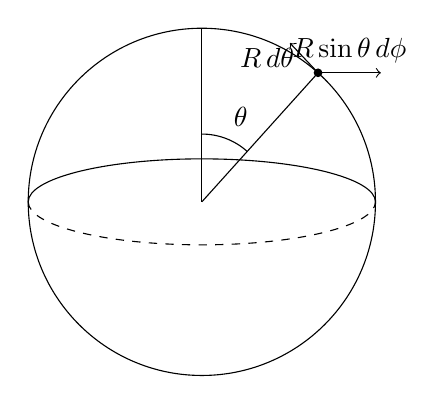
\begin{tikzpicture}[scale=1.05]
  \draw (0,0) circle (2.1);
  \draw[dashed] (-2.1,0) arc (180:360:2.1 and 0.52);
  \draw (2.1,0) arc (0:180:2.1 and 0.52);
  \coordinate (P) at (48:2.1);
  \fill (P) circle (1.5pt);
  \draw (0,0) -- (0,2.1);
  \draw (0,0) -- (P);
  \draw (0,0.82) arc (90:48:0.82);
  \node at (0.47,1.03) {\(\theta\)};
  \draw[->] (P) -- ++(-0.34,0.36)
    node[midway,left] {\(R\,d\theta\)};
  \draw[->] (P) -- ++(0.76,0)
    node[midway,above] {\(R\sin\theta\,d\phi\)};
\end{tikzpicture}
\caption{إعادة بناء واضحة للضلعين التفاضليين المحليين المستخدمين للحصول على \eqref{eq:sphere-metric}.}
\end{figure}

لا يوجد تحويل إحداثي شامل يحول \eqref{eq:sphere-metric} إلى مصفوفة إقليدية ثابتة. ويمكن لمراقب ثنائي الأبعاد أن يكتشف ذلك جوهريًا: فمثلث كبير بما يكفي ومكوَّن من جيوديسيات يكون مجموع زواياه أكبر من \(180^\circ\). وبذلك نكون قد وصلنا إلى المعيار المفيد. فالمعاملات المتغيرة لا تدل بذاتها على الانحناء. والانحناء هو العائق أمام إيجاد إحداثيات تجعل المترية ثابتة في جميع أنحاء المنطقة قيد النظر.

\section{من الزمكان المنحني إلى علم الكونيات}

تسمح النسبية العامة للزمكان نفسه بأن يمتلك هذا الانحناء الجوهري. وقد تكون \(g_{\mu\nu}\) المعتمدة على الموضع مجرد أثر من آثار الإحداثيات، كما في الإحداثيات القطبية، لكن في زمكان منحنٍ حقًا لا يزيل أي تحويل إحداثي هذا التغير على نحو شامل.

\begin{figure}[H]
\centering
\includegraphics[width=0.70\textwidth]{lecture_08_figure_09.png}
\caption{الانتقال من أمثلة إحداثية خاصة إلى عنصر الخط العام في الزمكان \(ds^2=g_{\mu\nu}(x)dx^\mu dx^\nu\).}
\lectureframe{00:48:40}
\end{figure}

لن نحاول تناول المنظومة الكاملة لمعادلات أينشتاين. وبدلًا من ذلك، نقصر اهتمامنا على هندسات ملائمة لعلم الكونيات: فنفترض أن الفضاء متجانس على المقاييس الكبيرة بما يكفي، مع إمكان تغيّر الهندسة مع الزمن. ويعني التجانس ألا يتميز موضع عن آخر. ولا يعني ذلك أن الفضاء مسطح: فكل نقطة على الكرة مكافئة لغيرها، ومع ذلك فالكرة منحنية. ولا يعني أيضًا أنه عديم البنية على كل مقياس.

\begin{classroomqa}
\audiencequestion{كيف يمكن للكون أن يكون متجانسًا بينما تشكل المجرات عناقيد وصفائح وخيوطًا؟}
\lecturerresponse{يتعلق هذا الادعاء بالمقاييس الخشنة. فالنجوم والمجرات والعناقيد شديدة عدم التجانس. وعند مقارنة مناطق تمتد عبر مئات الملايين من السنين الضوئية، تميل تلك البنى في المتوسط نحو توزيع منتظم. والمبدأ الكوني فرضية عمل تجريبية، لا ضرورة منطقية؛ ويمكن لاختلافات منهجية كبيرة بما يكفي، بما في ذلك الاختلافات الاتجاهية في الخلفية الكونية، أن تدحضه.}
\end{classroomqa}

الفرضية الثانية على المقاييس الكبرى في هذه المحاضرة هي التسطح المكاني. فعند زمن كوني ثابت، تبدو المثلثات الكبيرة بما يكفي إقليدية: مجموع زواياها يساوي \(180^\circ\). وهذا قول عن هندسة الفضاء الثلاثي الأبعاد، لا بعدُ عن انحناء الزمكان الرباعي الأبعاد.

\begin{classroomqa}
\audiencequestion{ماذا يعني التزامن لنقاط تفصل بينها مسافات كونية، ما دام ضوؤها يصل إلينا في أزمنة مختلفة؟}
\lecturerresponse{لا نستطيع أن نضع قضبان قياس بين مجرات بعيدة أو أن نفحصها آنيًا. فنحن نتلقى الإشارات لاحقًا ونعيد بناء هندسة أحداث الانبعاث ضمن نموذج للزمكان. والإجراء غير مباشر، لكن كثيرًا من القياسات الهندسية في الفلك كذلك أيضًا. ويعني التسطح أن المثلثات الكبيرة المعاد بناؤها لا تُظهر أي زيادة زاوية أو نقص زاوي يمكن كشفه على المقياس الذي شملته المسوح.}
\end{classroomqa}

\section{الإحداثيات المواكبة وعامل القياس}

تخيل شبكة ديكارتية مرسومة على الجريان واسع النطاق للمجرات. تحتفظ كل مجرة بوسمها الإحداثي مع تمدد الشبكة. وهذا الوسم ليس مسافة بالمتر؛ بل هو عنوان. ويحوِّل عامل تحويل تابع للزمن الفواصل الإحداثية إلى فواصل فيزيائية.

\begin{figure}[H]
\centering
\begin{tikzpicture}[>=Latex,scale=0.86]
  \foreach \x in {0,0.65,1.3,1.95,2.6} {
    \draw[gray!65] (\x,0) -- (\x,2.2);
  }
  \foreach \y in {0,0.55,1.1,1.65,2.2} {
    \draw[gray!65] (0,\y) -- (2.6,\y);
  }
  \fill[blue!65!black] (0.65,0.55) circle (2pt);
  \fill[red!70!black] (1.95,1.65) circle (2pt);
  \node[below] at (1.3,-0.2) {comoving labels at \(t_1\)};
  \draw[->,very thick] (3.0,1.1) -- (4.0,1.1)
    node[midway,above] {\(a(t)\) grows};
  \foreach \x in {4.4,5.5,6.6,7.7,8.8} {
    \draw[gray!65] (\x,0) -- (\x,2.2);
  }
  \foreach \y in {0,0.55,1.1,1.65,2.2} {
    \draw[gray!65] (4.4,\y) -- (8.8,\y);
  }
  \fill[blue!65!black] (5.5,0.55) circle (2pt);
  \fill[red!70!black] (7.7,1.65) circle (2pt);
  \node[below] at (6.6,-0.2) {same labels at \(t_2\)};
\end{tikzpicture}
\caption{تبقى العناوين الإحداثية المواكبة ثابتة، بينما يزداد التباعد الفيزيائي لشبكة الإحداثيات.}
\end{figure}

يقتضي التجانس المكاني عامل التحويل نفسه في كل مكان عند زمن معطى. ويتيح التسطح المكاني أن يكون الجزء المكاني من المترية ديكارتيًا. وعندئذ يكون عنصر الخط
\begin{equation}
  d\tau^2
  =dt^2-a^2(t)\left(dx^2+dy^2+dz^2\right).
  \label{eq:flrw-flat}
\end{equation}
هذه هي المترية الكونية المتجانسة والمسطحة مكانيًا في الإحداثيات المواكبة. ويمكننا أن نختار \(x,y,z\) بلا أبعاد وأن نعطي \(a(t)\) أبعاد الطول. ويمكن لاصطلاح آخر أن يضع الأبعاد في الإحداثيات ويجعل \(a\) بلا أبعاد؛ فالمهم هو حاصل الضرب وحده.

\begin{figure}[H]
\centering
\includegraphics[width=0.76\textwidth]{lecture_08_figure_10.png}
\caption{المترية الكونية المسطحة مكانيًا كما اكتملت على اللوح، مع العامل المشترك \(a^2(t)\) الذي يضرب الاتجاهات المكانية الثلاثة كلها.}
\lectureframe{01:03:15}
\end{figure}

لو كان \(a\) ثابتًا، لأمكننا امتصاصه بإعادة تحجيم \(x,y,z\)، ولأصبحت \eqref{eq:flrw-flat} زمكان مينكوفسكي العادي بوحدات مختلفة. واعتماده على الزمن هو العنصر غير التافه.

\begin{classroomqa}
\audiencequestion{إذا كانت شبكة الإحداثيات تتمدد، فلماذا لا تتمدد معها قضبان المتر والذرات والمجرات؟}
\lecturerresponse{تصف المترية متوسط الجريان الكوني، لا قوةً تُكرِه كل منظومة مترابطة على اتباعه. فالقوى الكهرومغناطيسية تُبقي قضيب المتر والذرة متماسكين، والجاذبية الذاتية تُبقي المجرة متماسكة. وتتغلب آثار الترابط تلك على التمدد الخلفي الضعيف للغاية على المقاييس الصغيرة. ويمكن للمجرات القريبة أيضًا أن تنحرف عن تدفق هابل: فأندروميدا تنجذب نحو درب التبانة. وتُظهر الدراسات المفصلة للترابط المجرّي أن المادة المرئية وحدها غير كافية، وهذه إحدى الحجج لصالح المادة المظلمة.}
\end{classroomqa}

\begin{classroomqa}
\audiencequestion{لماذا لا يكون عامل القياس نفسه قوةً تدفع المجرات متباعدة؟}
\lecturerresponse{له أبعاد الطول في الاصطلاح الحالي، لا أبعاد القوة. تخيل قذيفة مدفع أُطلقت إلى أعلى. فبعد إطلاقها، تكون حركتها الصاعدة قصورية؛ وتُغيِّر الجاذبية تلك الحركة بإنقاص سرعتها أو بجذبها عائدةً. وبالمثل، فالتمدد حالة حركة. والسؤال الديناميكي هو كيف تُغيِّر الجاذبية والمصادر الأخرى \(\dot a\) و\(\ddot a\)، لا ما القوة المطلوبة للإبقاء على \(a\) متحركًا.}
\end{classroomqa}

كان التوقع القديم أن الجاذبية، بوصفها جاذبة، ينبغي أن تبطئ التمدد. وبحلول وقت هذه المحاضرة، كانت الأدلة الفلكية قد أظهرت أن التمدد الحديث يتسارع بدلًا من ذلك، وهو ما يعني أن الديناميكيات الكاملة تتضمن أكثر من مادة جاذبة عادية. ونؤجل هذه المسألة إلى أن يترسخ الإعداد الهندسي.

\section{قانون هابل}

لنأخذ مجرتين مواكبتين يكون فصلهما الإحداثي الثابت هو \(\Delta x\). وعند زمن كوني مشترك تكون المسافة الفيزيائية بينهما
\begin{equation}
  D(t)=a(t)\,\Delta x.
  \label{eq:physical-distance}
\end{equation}
نشتق مع إبقاء الوسوم المواكبة ثابتة:
\begin{align}
  V(t)
    &=\dot D(t)
      =\dot a(t)\,\Delta x \nonumber\\
    &=\frac{\dot a(t)}{a(t)}D(t).
  \label{eq:hubble-derivation}
\end{align}
ونعرِّف
\begin{equation}
  H(t)=\frac{\dot a(t)}{a(t)}.
  \label{eq:hubble-parameter}
\end{equation}
وعندئذٍ
\begin{equation}
  V(t)=H(t)D(t).
  \label{eq:hubble-law}
\end{equation}
وعند زمن كوني واحد، تسري القيمة نفسها لـ \(H(t)\) في كل مكان؛ وإلا لما كان الفضاء متجانسًا. وتتناسب سرعة التباعد طرديًا مع المسافة لأن كل فاصل في الشبكة المواكبة يتمدَّد بالمعدل الكسري نفسه.

\begin{figure}[H]
\centering
\includegraphics[width=0.73\textwidth]{lecture_08_figure_11.png}
\caption{المسافة الفيزيائية \(D=a\Delta x\) ومشتقتها الزمنية في الطريق إلى \(V=(\dot a/a)D\).}
\lectureframe{01:16:45}
\end{figure}

\begin{classroomqa}
\audiencequestion{بالنسبة إلى مجرة بعيدة، هل ينبغي حساب معلمة هابل الآن أم عند انبعاث الضوء المرصود؟}
\lecturerresponse{في الحقبة التي يجري وصفها. فضوء المجرة البعيدة ينقل إلينا قيمة أسبق للتمدد. والتحليل الجاد يجب أن يراعي الاعتماد الزمني لـ \(H\)؛ أما إدخال قيمة اليوم في كل مكان فليس إلا تقريبًا محليًا.}
\end{classroomqa}

\begin{classroomqa}
\audiencequestion{أين تكمن الوحدات في \(D=a\Delta x\)؟}
\lecturerresponse{من الملائم أن نعامل الوسم المواكب \(\Delta x\) على أنه بلا أبعاد وأن نجعل \(a\) يحمل بعد الطول. والتوزيع العكسي للأبعاد ممكن أيضًا. وفي كلتا الحالتين، تكون لـ \(H=\dot a/a\) أبعاد مقلوب الزمن.}
\end{classroomqa}

\section{الضوء في الإحداثيات المتوسعة}

يسلك الضوء مسارًا صفريًا. وعلى مثل هذا المسار ينعدم فاصل الزمن الخاص:
\begin{equation}
  d\tau^2=0.
\end{equation}

\begin{classroomqa}
\audiencequestion{لماذا يكون الفاصل صفريًا للضوء؟}
\lecturerresponse{هذه هي الهندسة المُعرِّفة لشعاع الضوء في النسبية. فكل راصد محلي في سقوط حر يقيس حركة الضوء بسرعة \(c=1\)، ولذلك يكون \(dt^2=d\ell^2\) محليًا وينعدم فاصل الزمكان. ولا يعني هذا أنه لا يمر أي زمن إحداثي على الراصد الذي يتلقى الضوء.}
\end{classroomqa}

بالنسبة إلى شعاع يتحرك فقط في اتجاه \(x\)، يكون
\begin{equation}
  0=dt^2-a^2(t)\,dx^2.
\end{equation}
وباختيار الشعاع الذي يتحرك نحو ازدياد \(x\)، نحصل على
\begin{equation}
  dt=a(t)\,dx,
  \qquad
  dx=\frac{dt}{a(t)},
  \qquad
  \frac{dx}{dt}=\frac{1}{a(t)}.
  \label{eq:null-ray}
\end{equation}

\begin{figure}[H]
\centering
\includegraphics[width=0.64\textwidth]{lecture_08_figure_12.png}
\caption{شرط الصفرية في المترية المتوسعة، ومعادلة الشعاع الضوئي الناتجة في الإحداثيات المواكبة \(dx=dt/a(t)\).}
\lectureframe{01:23:45}
\end{figure}

تتناقص السرعة الإحداثية \(dx/dt\) مع ازدياد عامل القياس. ولا يعني هذا أن الضوء يبطؤ محليًا. فكل وحدة من مسافة إحداثية مواكبة تمثل مسافة فيزيائية أكبر فأكبر، ولذلك تتغير القيمة العددية للسرعة الإحداثية بينما يظل كل قياس محلي يعطي \(c=1\).

\section{لماذا يهم الاعتماد على الزمن}

أصبح السؤال الهندسي المركزي الآن لا مفر منه: كيف يتغير \(a(t)\)؟ والمماثلة هنا هي مقذوف نعرف موضعه عند لحظة واحدة. فمساره المستقبلي يتطلب معادلة حركة. وفي علم الكونيات، ستزوِّدنا الديناميكيات الثقالية بالمعادلة الخاصة بـ \(a(t)\).

\begin{classroomqa}
\audiencequestion{لماذا نمنح سؤال ما إذا كان \(a(t)\) يتغير أولوية على السؤال المشروع بالقدر نفسه عمّا إذا كانت، مثلًا، شحنة الإلكترون تتغير مع الزمن؟}
\lecturerresponse{لا يوجد تراتب منطقي. وأي تغير مقيس في شحنة الإلكترون سيكون بالغ الأهمية. ونحن نركز على \(a(t)\) لأن الرصد يخبرنا بالفعل بأن الفواصل الكونية تتغير، في حين تبدو شحنة الإلكترون ثابتة. ومن الناحية الهندسية، يمكن إزالة \(a\) الثابت بتغيير الوحدات المكانية، وسيترك ذلك زمكانًا مسطحًا؛ أما \(a\) المعتمد على الزمن فلا يمكن إزالته بهذه الطريقة.}
\end{classroomqa}

قبل قياس تباعد الأجرام البعيدة، نحتاج إلى هذا الإطار الهندسي لكي نحدد ما الذي يُقاس. وعلى أبسط مستوى، يبدو المصدر ذو اللمعان المعلوم أخفت مع ازدياد المسافة لأن ضوءه ينتشر على مساحة أكبر، بينما تعطي إزاحة الخطوط الطيفية الذرية المعلومة انزياحًا نحو الأحمر، ومن ثم مؤشرًا على التباعد. جمع هابل بين تقديرات المسافة والانزياحات نحو الأحمر لاكتشاف التناسب \eqref{eq:hubble-law}، مع أن القيمة العددية المبكرة للمعامل كانت خاطئة إلى حد كبير. أما سلالم المسافات الحديثة وحسابات انتشار الضوء النسبية فأكثر تعقيدًا بكثير، لكن الزوج المفهومي يبقى هو المسافة مع الانزياح نحو الأحمر.

\section{زمن هابل وتقدير العمر}

توجد قيمة تقديرية بسيطة كامنة في قانون هابل. إذا ثبّتنا سرعة تباعد مجرة ما الحالية وأرجعنا الحركة إلى الخلف على نحو منتظم، فإن الزمن اللازم لسد مسافتها الحالية سيكون
\begin{equation}
  t=\frac{D}{V}.
\end{equation}
وباستخدام \(V=HD\)، نحصل على
\begin{equation}
  t=\frac{D}{HD}=\frac{1}{H}.
  \label{eq:hubble-time}
\end{equation}
تُلغى المسافة، ولذلك يعطي كل زوج من المجرات المتسايرة الزمن التقريبي نفسه. يلتقط ساسكيند هنا خطأً لفظيًا يسيرًا ويصححه. فالافتراض ليس أن \(H\) يبقى ثابتًا. وإنما الافتراض هو استقراء سرعة التباعد المعينة تلك إلى الخلف كما لو كانت ثابتة.

\begin{figure}[H]
\centering
\includegraphics[width=0.66\textwidth]{lecture_08_figure_13.png}
\caption{تقدير زمن هابل \(H^{-1}=D/(HD)=D/V\)، حيث تُلغى المسافة في الاستقراء إلى الخلف.}
\lectureframe{01:33:45}
\end{figure}

لذلك فإن مقلوب معامل هابل هو مقياس زمني، وليس بالضرورة العمر الدقيق للكون. ففي صورة متباطئة صرفًا يهيمن عليها المادة، اعكس السرعة الحالية ودع الجاذبية تجذب المجرات بعضها إلى بعض. عندئذ تلتقي أبكر مما لو تحركت بسرعة منتظمة، ولذلك فإن \(H^{-1}\) المحسوب اليوم يبالغ في تقدير العمر. وتذكر المحاضرة عمرًا منقحًا يقارب \(13.5\) مليار سنة، وهو قريب من زمن هابل لكنه غير مطابق له.

\begin{classroomqa}
\audiencequestion{إذا لم يكن داخل مجرتنا تمدد هابل، فما معنى أن نرجع جميع المجرات إلى الخلف حتى تنهار؟}
\lecturerresponse{إن الوصف المتجانس يكف في النهاية عن تمثيل التاريخ الحقيقي للبنى المرتبطة. فإلى الأمام في الزمن تنمو التقلبات الصغيرة ثقاليًا لتصير مجرات وعناقيد. أما الفيلم المعكوس حرفيًا فسيتطلب أن تنعكس كل حركة مجهرية وأن تنخفض الإنتروبيا؛ ومجرد عكس تدفق هابل المتوسط لا يبطل تشكل البنية. والاستقراء إلى الخلف تقدير كوني خشن، لا فيلمًا تعيد فيه كل نجمة اقتفاء مسارها.}
\end{classroomqa}

\begin{classroomqa}
\audiencequestion{هل يمكن لتجربة أن تميز بين تزايد المسافة بين المجرات وانكماش مسطرة؟}
\lecturerresponse{المقادير القابلة للرصد هي النسب عديمة الأبعاد فقط. وما يُقاس هو أن المسافة بين المجرات مقسومة على معيار طولي ذري أو مختبري تزداد. ونثبت اصطلاحًا معاملات الفيزياء الذرية والجزيئية ونقول إن الكون يتمدد. ويمكن للمرء أن يختار الفصل بين المجرات معيارًا ويصف الذرات والبروتونات وقضبان المتر بأنها تنكمش. ولن تتغير فيزياء النسبة.}
\end{classroomqa}

وهذا الاصطلاح طبيعي لأن قضبان القياس مكوّنة من ذرات، ويتحكم في حجمها معاملات تبدو ثابتة. فالمتر هو في نهاية المطاف عدد كبير من الأطوال المجهرية. وتثبيت تلك المعايير المجهرية يعطينا العبارة المألوفة بأن \(a(t)\) يزداد.

\begin{classroomqa}
\audiencequestion{هل \eqref{eq:flrw-flat} هي المترية الوحيدة المتوافقة مع التجانس المكاني والاستواء؟}
\lecturerresponse{فقط حتى تحويلات الإحداثيات. والقول الدقيق هو أنه، تحت هذه الافتراضات ومع اختيار مناسب للزمن الكوني وللإحداثيات المكانية المتسايرة، يمكن جلب المترية إلى هذه الصورة. وقد يجعل نظام إحداثيات آخر الزمكان نفسه يبدو مختلفًا تمامًا.}
\end{classroomqa}

\begin{classroomqa}
\audiencequestion{عندما يصل الانفصال عند الاستقراء إلى الخلف إلى الصفر، يعطي قانون هابل أيضًا سرعة صفرية. فهل يمنع ذلك المجرات من الالتقاء؟}
\lecturerresponse{لا. إن \(H\) المستنتج اليوم لا يُفترض ثباته على طول الطريق إلى الماضي. ففي الحلول التمددية الاعتيادية كان \(H(t)\) أكبر بكثير في الأزمنة الأسبق. ويُجرى التقدير \(H_0^{-1}\) بمدّ سرعة اليوم بانتظام لمجرد الحصول على مقياس؛ أما \(a(t)\) و\(H(t)\) والسرعات الحقيقية فيجب إيجادها من الديناميات.}
\end{classroomqa}

\section{مبرهنة نيوتن للغلاف والديناميات الكونية}

لاكتشاف الديناميات، استعض عن المجرات بوسط متجانس. اختر مجرةً واحدة أصلًا، وأخرى ذات المعلمة المتسايرة \(x\). ولا امتياز فيزيائيًا في هذا الاختيار؛ فالتجانس يقتضي أن تكون المعادلة النهائية هي نفسها حول كل مجرة. ونصف القطر الفيزيائي للمجرة الثانية هو
\begin{equation}
  R(t)=a(t)x.
  \label{eq:radius-ax}
\end{equation}

في البداية، يبدو أن إيجاد تسارعها الثقالي يقتضي جمع قوى الجذب الصادرة عن كل مجرة في كون هائل. لكن مبرهنة نيوتن للغلاف تختزل المسألة:

\begin{proposition}[Newton's shell theorem]
بالنسبة إلى قوة تتناقص مع مربع المسافة وتوزيع كتلي ذي تناظر كروي، فإن المادة الواقعة خارج كرة تمر بنقطة الاختبار تسهم بمحصل قوة تساوي الصفر. أما المادة داخل الكرة فتؤثر في نقطة الاختبار كما لو كانت الكتلة المحصورة كلها متمركزة في المركز.
\end{proposition}

\begin{figure}[H]
\centering
\includegraphics[width=0.70\textwidth]{lecture_08_figure_14.png}
\caption{توزيع المجرات المتجانس، ومجرة اختبار عند المعلمة المتسايرة \(x\)، والكرة التي تتحكم كتلتها المحصورة وحدها في حركتها الشعاعية.}
\lectureframe{01:50:05}
\end{figure}

\begin{figure}[H]
\centering
\begin{tikzpicture}[scale=0.94,>=Latex]
  \draw[gray!65] (0,0) circle (2.35);
  \foreach \p in {
    (-1.5,0.8),(-1.2,-0.8),(-0.8,1.5),(-0.6,0.35),(-0.3,-1.45),
    (0.15,1.05),(0.35,-0.55),(0.7,1.65),(0.9,0.45),(1.25,-0.9),
    (1.65,0.95),(-1.75,-0.2),(1.8,-0.15)} {
    \fill[black!55] \p circle (1.15pt);
  }
  \fill[blue!65!black] (0,0) circle (2pt)
    node[below left] {chosen origin};
  \fill[red!70!black] (2.35,0) circle (2.2pt)
    node[right] {test galaxy};
  \draw[->,thick] (0,0) -- (2.32,0)
    node[midway,above] {\(R=a(t)x\)};
  \draw[<->] (-2.35,-2.55) -- (2.35,-2.55)
    node[midway,below=4pt] {only the enclosed mass contributes};
\end{tikzpicture}
\caption{إعادة بناء منقحة لإعداد مبرهنة الغلاف. والأصل اختيار ملائم، لا مركزًا للكون.}
\end{figure}

وهكذا تحولت مسألة الأجسام المتعددة الكونية إلى مسألة مألوفة لجسم واحد: جسم يتحرك شعاعيًا تحت جذب الكتلة المحصورة داخل كرته الحالية. وستحدد معادلة نيوتن كيف يتسارع \(R=a x\)، ومن ثم \(a(t)\). وتتوقف المحاضرة عمدًا قبل إجراء ذلك الحساب. وفي اللقاء التالي سيُشتق أبسط كونيات تهيمن عليها المادة، بدلًا من دس جوابها في الإعداد الهندسي.

\section{أسئلة متأخرة: الضوء، والانفجار العظيم، والانحناء}

انتهت المحاضرة الرسمية، لكن الأسئلة الأخيرة تكشف عدة تصورات مضللة، وهي جزء من الفيزياء لا مجرد ملحق.

\begin{classroomqa}
\audiencequestion{إذا كان ضوء الأجسام البعيدة جدًا قد انبعث حين كان الكون أصغر بكثير، فلماذا يبدو الآن آتيًا من مسافة بعيدة إلى هذا الحد؟ وإذا كان الكون المبكر متراصًا، فلماذا لا يكون كله قابلًا للرصد؟}
\lecturerresponse{يجب حل معادلة الشعاع الصفري في الإحداثيات المتوسعة. فعندما يكون \(a(t)\) صغيرًا جدًا، يكون \(dx/dt=1/a(t)\) كبيرًا جدًا: يقطع الضوء فاصلًا متسايرًا كبيرًا مع أنه لا يزال يتحرك محليًا بسرعة \(c=1\). ومع ازدياد \(a(t)\)، تنخفض سرعته الإحداثية. وتعتمد نقطة الانبعاث الدقيقة وحجم المنطقة القابلة للرصد على التاريخ الكامل لـ\(a(t)\)، ولذلك يؤجَّل الجواب العددي إلى أن يُحل نموذج كوني محدد.}
\end{classroomqa}

\begin{figure}[H]
\centering
\includegraphics[width=0.72\textwidth]{lecture_08_figure_15.png}
\caption{شعاع ضوئي في المستوى \((x,t)\): يكون شبه أفقي في الإحداثيات المتسايرة عندما يكون \(a(t)\) صغيرًا، ثم يزداد انحدارًا تدريجيًا مع نمو عامل القياس.}
\lectureframe{01:56:20}
\end{figure}

إن تكامل \eqref{eq:null-ray} يجعل الحساب المؤجَّل صريحًا:
\begin{equation}
  \Delta x
  =\int_{t_{\mathrm e}}^{t_0}\frac{dt}{a(t)}.
  \label{eq:comoving-light-distance}
\end{equation}
وما إذا كان التكامل يبلغ مسافات متسايرة كبيرة بلا حد عندما يقترب \(t_{\mathrm e}\) من البداية يعتمد على الصيغة المبكرة لـ\(a(t)\).\editorialnote{المعادلة \eqref{eq:comoving-light-distance} هي الصيغة المتكاملة للمعادلة المكتوبة على اللوح \(dx=dt/a(t)\). وهي تُظهر صراحةً الحساب الذي تُحيله المحاضرة إلى اللقاء التالي من غير اختيار عامل قياس بعينه.}

\begin{figure}[H]
\centering
\begin{tikzpicture}[scale=0.92,>=Latex]
  \draw[->] (0,0) -- (6.4,0) node[right] {\(x\)};
  \draw[->] (0,0) -- (0,4.6) node[above] {\(t\)};
  \draw[thick,blue!65!black]
    plot[smooth] coordinates {(0,0.18) (1.65,0.42) (2.65,1.05)
      (3.35,2.05) (3.85,3.25) (4.05,4.25)};
  \fill[red!70!black] (4.05,4.25) circle (2pt)
    node[right] {reception today};
  \draw[dashed] (4.05,0) -- (4.05,4.25);
  \node[align=left] at (1.65,3.25)
    {\(\displaystyle \frac{dx}{dt}=\frac1{a(t)}\)\\
     large when \(a\) is small};
\end{tikzpicture}
\caption{نسخة منقحة لبناء الشعاع الضوئي في الإحداثيات المتسايرة. وتغيّر الميل أثر إحداثي، لا تغيّرًا في السرعة المحلية للضوء.}
\end{figure}

\begin{classroomqa}
\audiencequestion{هل قذف الانفجار العظيم المادة من نقطة واحدة بحيث ينبغي لها الآن أن تقع على غلاف متمدد أو حلقة متمددة؟}
\lecturerresponse{لا. يبدأ النموذج بفضاء متجانس شديد الكثافة للغاية. فكل تباعد على المقاييس الكبيرة يزداد؛ والمادة لا تُقذف عبر فراغ موجود سلفًا من مركز مميز. والبالون المغطى على نحو منتظم بنقاط هو تشبيه ثنائي الأبعاد مفيد: فمع تمدده، تزداد جميع المسافات الفاصلة بين النقاط بينما يبقى سطحه مغطى بالنقاط على نحو متجانس. وقد يكون الفضاء لا نهائيًا حتى عند كل زمن موجب؛ فالتمدد لا يعني أنه بدأ كرة منتهية داخل شيء آخر.}
\end{classroomqa}

\begin{classroomqa}
\audiencequestion{هل كانت الجاذبية نفسها أضعف أم أقوى أثناء التمدد؟}
\lecturerresponse{يفترض هذا النقاش أن ثابت نيوتن \(G\) ثابت. ومع ذلك تتغير القوة لأن المسافات الفاصلة والكثافات المحصورة تتغير. وفي وقت أبكر، كانت المجرة المواكبة نفسها أقرب فعليًا، وكانت المادة المتجانسة أشد كثافة، لذلك كان التباطؤ الثقالي أكبر. وهذا هو بالضبط ما يُراد من حساب مبرهنة القشرة أن يحدده كمّيًا.}
\end{classroomqa}

أخيرًا، يجب ألا يُخلط بين الانحناء المكاني والتمدد. تبدو رقعة صغيرة من الأرض مسطحة لأن حجمها صغير جدًا مقارنة بنصف قطر الأرض. وبقياس مثلثات كبيرة بما يكفي، يمكن للمرء إما أن يكتشف فائضًا زاويًا أو أن يضع حدًا أدنى لنصف قطر الانحناء. ويجري علم الفلك التجربة المناظرة بمثلثات هائلة. وبلغة الرصد المستخدمة في محاضرة 2006، لم يُكتشف أي انحناء على امتداد الجزء المرئي، لذا كان لا بد أن يكون أي نصف قطر للانحناء أكبر بكثير منه. وهذا لا يثبت كونًا مسطحًا تمامًا؛ بل يضع حدًا لمدى انحناء الجزء المتاح.

بالنسبة إلى كرة، يتناسب الانحناء الجوهري مع \(R^{-2}\). ولذلك تصبح الكرة النامية أكثر تسطحًا محليًا. وبالمثل، إذا كان لكون متجانس انحناء مكاني غير صفري، فإن التمدد يزيد نصف قطر انحنائه ويقلل الانحناء المرئي في أي رقعة محلية ثابتة الحجم.
\editorialnote{إن التناسب \(R^{-2}\) هو الصيغة الكمية القياسية لقول المحاضرة إن القيمة العددية للانحناء تتناقص مع نمو الكرة.}

\begin{classroomqa}
\audiencequestion{إذا كان الفضاء منحنياً، فهل يجب أن يكون أحد مكونات الكون منكمشًا بينما يتمدد مكوّن آخر؟}
\lecturerresponse{لا. فالانحناء المكاني الموجب أو الصفري أو السالب يصف هندسة كل شريحة من الزمن الكوني. ويتحكم تطور \(a(t)\) في التمدد أو الانكماش. يمكن لكون منحنٍ أن يتمدد؛ ويمكن لكون مسطح أن ينكمش. وقد ينعكس التمدد لاحقًا، تمامًا كما قد يسقط مقذوف صاعد عائدًا، لكن انكماشًا متزامنًا ليس كامنًا داخل الانحناء. والمسألة الديناميكية هي ما إذا كانت الحركة إلى الخارج تفلت من جذب الكتلة المحصورة، أو ترتد راجعة، أو تقع على الحد الحرج.}
\end{classroomqa}

تلك المقارنة بسرعة الإفلات هي آخر فكرة تُعرض على اللوح في المحاضرة. لقد زودتنا الهندسة بالمترية، وقانون هابل، ومعادلة شعاع الضوء. واختزلت مبرهنة نيوتن الديناميكيات إلى الكتلة داخل كرة واحدة. وتبدأ المحاضرة التالية تمامًا حيث ينبغي أن تنتهي هذه: بالمعادلة التي تحدد \(a(t)\)، وبسؤال ما إذا كان التمدد يفلت، أو يعاود الانهيار، أو يقع على الحد الحرج.
